\documentclass[11pt,a4paper]{article}
\usepackage[utf8]{inputenc}
\usepackage[T1]{fontenc}
\usepackage{geometry}
\usepackage{graphicx}
\usepackage{xcolor}
\usepackage{listings}
\usepackage{fancyhdr}
\usepackage{titlesec}
\usepackage{hyperref}
\usepackage{tikz}
\usepackage{amsmath}
\usepackage{amssymb}
\usepackage{enumitem}
\usepackage{booktabs}
\usepackage{float}

% Page setup
\geometry{margin=1in}
\pagestyle{fancy}
\fancyhf{}
\fancyhead[L]{C Programming for Post-Silicon Validation}
\fancyhead[R]{\thepage}
\fancyfoot[C]{6-Day Intensive Course Manual}

% Colors
\definecolor{codeblue}{RGB}{0,102,204}
\definecolor{codegray}{RGB}{128,128,128}
\definecolor{codegreen}{RGB}{0,128,0}
\definecolor{backcolour}{RGB}{245,245,245}

% Code listing style
\lstdefinestyle{cstyle}{
    backgroundcolor=\color{backcolour},
    commentstyle=\color{codegreen},
    keywordstyle=\color{codeblue},
    numberstyle=\tiny\color{codegray},
    stringstyle=\color{red},
    basicstyle=\ttfamily\footnotesize,
    breakatwhitespace=false,
    breaklines=true,
    captionpos=b,
    keepspaces=true,
    numbers=left,
    numbersep=5pt,
    showspaces=false,
    showstringspaces=false,
    showtabs=false,
    tabsize=2,
    frame=single,
    rulecolor=\color{black}
}

\lstset{style=cstyle}

% Title formatting
\titleformat{\section}{\Large\bfseries\color{codeblue}}{\thesection}{1em}{}
\titleformat{\subsection}{\large\bfseries}{\thesubsection}{1em}{}

\hypersetup{
    colorlinks=true,
    linkcolor=codeblue,
    filecolor=magenta,
    urlcolor=cyan,
    pdftitle={C Programming for Post-Silicon Validation - Course Manual},
    pdfauthor={Course Instructor},
}

\begin{document}

% Title Page
\begin{titlepage}
    \centering
    \vspace*{2cm}

    {\Huge\bfseries C Programming for\\Post-Silicon Validation Engineers\par}
    \vspace{1cm}
    {\Large 6-Day Intensive Course Manual\par}
    \vspace{2cm}

    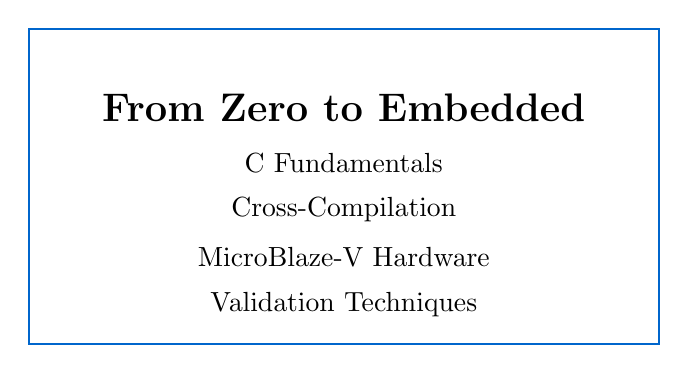
\begin{tikzpicture}
        \draw[codeblue, thick] (0,0) rectangle (8,4);
        \node at (4,3) {\Large\textbf{From Zero to Embedded}};
        \node at (4,2.3) {C Fundamentals};
        \node at (4,1.7) {Cross-Compilation};
        \node at (4,1.1) {MicroBlaze-V Hardware};
        \node at (4,0.5) {Validation Techniques};
    \end{tikzpicture}

    \vspace{2cm}
    {\large Designed for 20 Engineers\\No Prior Coding Experience Required\par}
    \vspace{1cm}
    {\large Version 1.0 - 2025\par}

    \vfill

    {\large Course Duration: 6 Days (42 Hours)\\
    Target Audience: Post-Silicon Validation Engineers\\
    Hardware Platform: AMD MicroBlaze-V (RISC-V)\par}
\end{titlepage}

\newpage
\tableofcontents
\newpage

\section{Executive Summary}

This comprehensive 6-day course transforms engineers with no coding experience into proficient C programmers capable of developing embedded validation tools for semiconductor post-silicon testing. The curriculum emphasizes hands-on learning with real hardware (MicroBlaze-V-based FPGA) and industry-standard tooling.

\subsection{Course Objectives}
By the end of this course, participants will be able to:
\begin{itemize}
    \item Write, compile, and debug C programs using GCC and GDB
    \item Cross-compile code for RISC-V processors
    \item Develop embedded applications for the MicroBlaze-V platform
    \item Implement validation routines simulating post-silicon testing scenarios
    \item Use GitHub for version control and collaborative development
    \item Apply AI tools responsibly for code assistance and debugging
\end{itemize}

\subsection{Key Features}
\begin{itemize}
    \item \textbf{Validation-Focused}: All examples simulate real-world post-silicon scenarios
    \item \textbf{Hands-On Learning}: 60\% lab time with scaffolded GitHub Classroom assignments
    \item \textbf{Progressive Complexity}: From basic syntax to embedded hardware programming
    \item \textbf{Industry Tools}: GCC, GDB, GitHub, VS Code, RISC-V Toolchain
    \item \textbf{AI Integration}: Responsible introduction of AI coding assistants
    \item \textbf{Portfolio Building}: GitHub-based projects for professional development
\end{itemize}

\section{Prerequisites and Preparation}

\subsection{Target Audience}
\begin{itemize}
    \item 20 engineers transitioning to post-silicon validation roles
    \item No prior programming experience required
    \item Basic understanding of digital electronics and semiconductors assumed
    \item Familiarity with command-line interfaces helpful but not required
\end{itemize}

\subsection{Pre-Course Requirements}
Participants must complete the following setup 1 week before the course:

\subsubsection{Tool Installation}
\begin{enumerate}
    \item \textbf{Development Environment}
    \begin{itemize}
        \item GCC compiler (native)
        \item RISC-V cross-compiler (riscv64-unknown-elf-gcc)
        \item CMake (version 3.13+)
        \item Git version control
        \item VS Code with C/C++ extension
    \end{itemize}

    \item \textbf{RISC-V Development Tools}
    \begin{itemize}
        \item RISC-V GNU Toolchain (latest version)
        \item Python 3.x for build scripts
        \item QEMU RISC-V emulator (virt machine) for fallback simulation
    \end{itemize}

    \item \textbf{Debugging Tools}
    \begin{itemize}
        \item GDB debugger
        \item OpenOCD (for hardware debugging)
    \end{itemize}
\end{enumerate}

\subsubsection{Knowledge Prerequisites}
\begin{itemize}
    \item Complete Git tutorial (2 hours): clone, commit, push, pull requests
    \item Watch CS50 C introduction videos (first 2 lectures)
    \item Read RISC-V GPIO and memory-mapped I/O documentation overview
\end{itemize}

\section{Daily Curriculum Overview}

\subsection{Day 1: C Fundamentals and Compilation}

\textbf{Learning Objectives:}
\begin{itemize}
    \item Understand C syntax and basic data types
    \item Learn compilation process with GCC
    \item Write simple validation calculations
\end{itemize}

\textbf{Topics Covered:}
\begin{itemize}
    \item Variables and data types (int, float, char)
    \item Operators and expressions
    \item Input/output with printf/scanf
    \item GCC compilation flags and error handling
\end{itemize}

\textbf{Validation Context:}
Programs simulate basic chip parameter validation, such as voltage threshold checking and power calculations.

\begin{lstlisting}[language=C, caption=Day 1 Example: Voltage Validator]
#include <stdio.h>

int main() {
    float voltage, current, power;
    float min_voltage = 1.8;
    float max_voltage = 3.3;

    printf("Enter supply voltage (V): ");
    scanf("%f", &voltage);

    printf("Enter current (A): ");
    scanf("%f", &current);

    // Validate voltage range
    if (voltage < min_voltage || voltage > max_voltage) {
        printf("ERROR: Voltage %.2fV out of range [%.1f-%.1f]V\n",
               voltage, min_voltage, max_voltage);
        return 1;
    }

    power = voltage * current;
    printf("Power consumption: %.3fW\n", power);
    printf("Validation: PASS\n");

    return 0;
}
\end{lstlisting}

\subsection{Day 2: Control Flow and Debugging}

\textbf{Learning Objectives:}
\begin{itemize}
    \item Master conditional statements and loops
    \item Learn function definition and calling
    \item Use GDB for debugging
\end{itemize}

\textbf{Topics Covered:}
\begin{itemize}
    \item if-else statements and logical operators
    \item for and while loops
    \item Function declaration, definition, and parameters
    \item GDB basics: breakpoints, stepping, variable inspection
\end{itemize}

\textbf{Validation Context:}
Implement test sequences that repeatedly check register values and detect fault conditions.

\begin{lstlisting}[language=C, caption=Day 2 Example: Register Monitor]
#include <stdio.h>

// Simulate reading a hardware register
int read_register(int address) {
    // In real hardware, this would access memory-mapped I/O
    static int sim_values[] = {0x1234, 0x5678, 0x9ABC, 0xDEF0};
    return sim_values[address % 4];
}

int validate_register_sequence(int start_addr, int count) {
    int errors = 0;

    for (int i = 0; i < count; i++) {
        int addr = start_addr + i;
        int value = read_register(addr);

        printf("Register 0x%04X: 0x%04X\n", addr, value);

        // Check for invalid patterns (all zeros or all ones)
        if (value == 0x0000 || value == 0xFFFF) {
            printf("  WARNING: Suspicious value detected!\n");
            errors++;
        }
    }

    return errors;
}

int main() {
    int base_address = 0x1000;
    int register_count = 8;

    printf("Starting register validation...\n");
    int error_count = validate_register_sequence(base_address, register_count);

    if (error_count == 0) {
        printf("Validation PASSED: All registers OK\n");
    } else {
        printf("Validation FAILED: %d errors detected\n", error_count);
    }

    return error_count;
}
\end{lstlisting}

\subsection{Day 3: Memory Management and Data Structures}

\textbf{Learning Objectives:}
\begin{itemize}
    \item Understand pointers and memory addressing
    \item Work with arrays and strings
    \item Use structures to model hardware components
    \item Learn bit manipulation for register operations
\end{itemize}

\textbf{Topics Covered:}
\begin{itemize}
    \item Pointer declaration, dereferencing, and arithmetic
    \item Arrays and string handling
    \item Structures and typedef
    \item Bit operations: AND, OR, XOR, shifts
    \item Memory safety and common pitfalls
\end{itemize}

\textbf{Validation Context:}
Model chip components as structures and manipulate register bits to simulate hardware control.

\begin{lstlisting}[language=C, caption=Day 3 Example: Chip State Monitor]
#include <stdio.h>
#include <stdint.h>

// Structure to represent a chip's state
typedef struct {
    uint32_t control_reg;
    uint32_t status_reg;
    uint32_t error_reg;
    char chip_id[16];
    float temperature;
} ChipState;

// Bit manipulation macros
#define SET_BIT(reg, bit)    ((reg) |= (1U << (bit)))
#define CLEAR_BIT(reg, bit)  ((reg) &= ~(1U << (bit)))
#define CHECK_BIT(reg, bit)  (((reg) >> (bit)) & 1U)

void print_chip_state(ChipState *chip) {
    printf("Chip ID: %s\n", chip->chip_id);
    printf("Temperature: %.1f°C\n", chip->temperature);
    printf("Control Register: 0x%08X\n", chip->control_reg);
    printf("Status Register:  0x%08X\n", chip->status_reg);
    printf("Error Register:   0x%08X\n", chip->error_reg);

    // Check specific status bits
    printf("Power Status: %s\n",
           CHECK_BIT(chip->status_reg, 0) ? "ON" : "OFF");
    printf("Clock Status: %s\n",
           CHECK_BIT(chip->status_reg, 1) ? "LOCKED" : "UNLOCKED");
    printf("Error Status: %s\n",
           CHECK_BIT(chip->error_reg, 0) ? "ERROR" : "OK");
}

int validate_chip_array(ChipState chips[], int count) {
    int failed_chips = 0;

    for (int i = 0; i < count; i++) {
        printf("\n--- Chip %d ---\n", i);
        print_chip_state(&chips[i]);

        // Validation checks
        if (chips[i].temperature > 85.0) {
            printf("FAIL: Temperature too high!\n");
            failed_chips++;
        }

        if (CHECK_BIT(chips[i].error_reg, 0)) {
            printf("FAIL: Error bit set!\n");
            failed_chips++;
        }
    }

    return failed_chips;
}
\end{lstlisting}

\subsection{Day 4: Advanced Functions and Cross-Compilation}

\textbf{Learning Objectives:}
\begin{itemize}
    \item Organize code with modular functions
    \item Understand cross-compilation for embedded targets
    \item Introduction to the Pico SDK
    \item Set up CMake build system
\end{itemize}

\textbf{Topics Covered:}
\begin{itemize}
    \item Function scope, static variables, and header files
    \item Cross-compilation with arm-none-eabi-gcc
    \item Pico SDK initialization and basic structure
    \item CMake configuration for embedded projects
\end{itemize}

\textbf{Validation Context:}
Create modular test functions that can be compiled for both native debugging and ARM target deployment.

\begin{lstlisting}[language=C, caption=Day 4 Example: CMakeLists.txt for Pico]
cmake_minimum_required(VERSION 3.13)

# Include the Pico SDK
include($ENV{PICO_SDK_PATH}/external/pico_sdk_import.cmake)

project(validation_suite C CXX ASM)

set(CMAKE_C_STANDARD 11)
set(CMAKE_CXX_STANDARD 17)

# Set RISC-V toolchain
set(CMAKE_C_COMPILER riscv64-unknown-elf-gcc)
set(CMAKE_CXX_COMPILER riscv64-unknown-elf-g++)

# Add executable
add_executable(validation_suite
    src/main.c
    src/register_tests.c
    src/gpio_tests.c
    src/timing_tests.c
)

# RISC-V specific flags
target_compile_options(validation_suite PRIVATE
    -march=rv32i
    -mabi=ilp32
    -mcmodel=medlow
)

# Link libraries (standard C library for RISC-V)
target_link_libraries(validation_suite
    c
    m
)

# Create binary and hex files for FPGA deployment
add_custom_command(TARGET validation_suite POST_BUILD
    COMMAND ${CMAKE_OBJCOPY} -O binary $<TARGET_FILE:validation_suite> validation_suite.bin
    COMMAND ${CMAKE_OBJCOPY} -O ihex $<TARGET_FILE:validation_suite> validation_suite.hex
)
\end{lstlisting}

\subsection{Day 5: Hardware Debugging and MicroBlaze-V Peripherals}

\textbf{Learning Objectives:}
\begin{itemize}
    \item Advanced GDB debugging techniques
    \item MicroBlaze-V GPIO and peripheral control
    \item Hardware-in-the-loop testing concepts
    \item Fault injection and detection
\end{itemize}

\textbf{Topics Covered:}
\begin{itemize}
    \item GDB with embedded targets
    \item GPIO initialization and control
    \item ADC for sensor simulation
    \item Timer-based testing
    \item USB communication for test results
\end{itemize}

\textbf{Validation Context:}
Implement actual hardware tests using MicroBlaze-V peripherals to simulate post-silicon validation scenarios.

\begin{lstlisting}[language=C, caption=Day 5 Example: GPIO Validation Test]
#include <stdio.h>
#include <stdint.h>
#include <stdbool.h>
#include <unistd.h>

#define LED_PIN 25
#define TEST_PIN_START 2
#define TEST_PIN_COUNT 8

typedef struct {
    uint8_t pin;
    bool expected_state;
    bool actual_state;
    bool passed;
} gpio_test_result_t;

void init_test_hardware(void) {
    // Initialize UART for stdio
    printf("Initializing RISC-V FPGA test hardware...\n");

    // Initialize GPIO memory-mapped registers
    // Base addresses would be defined in hardware specification
    volatile uint32_t *gpio_base = (volatile uint32_t *)0x10012000;

    // Configure LED pin as output
    gpio_base[GPIO_OUTPUT_EN] |= (1 << LED_PIN);

    // Configure test pins as outputs
    for (int i = 0; i < TEST_PIN_COUNT; i++) {
        gpio_base[GPIO_OUTPUT_EN] |= (1 << (TEST_PIN_START + i));
    }
}

int run_gpio_validation_suite(gpio_test_result_t results[]) {
    int passed_tests = 0;

    printf("Starting GPIO validation suite...\n");

    for (int i = 0; i < TEST_PIN_COUNT; i++) {
        uint8_t pin = TEST_PIN_START + i;

        // Test high output
        gpio_put(pin, 1);
        sleep_ms(10);
        bool high_state = gpio_get(pin);

        // Test low output
        gpio_put(pin, 0);
        sleep_ms(10);
        bool low_state = gpio_get(pin);

        // Record results
        results[i].pin = pin;
        results[i].expected_state = true;
        results[i].actual_state = high_state && !low_state;
        results[i].passed = results[i].actual_state;

        if (results[i].passed) {
            passed_tests++;
            printf("Pin %d: PASS\n", pin);
        } else {
            printf("Pin %d: FAIL (High: %d, Low: %d)\n",
                   pin, high_state, low_state);
        }

        // Blink LED to show progress
        gpio_put(LED_PIN, 1);
        sleep_ms(100);
        gpio_put(LED_PIN, 0);
        sleep_ms(100);
    }

    return passed_tests;
}

int main() {
    gpio_test_result_t test_results[TEST_PIN_COUNT];

    init_test_hardware();

    printf("RISC-V FPGA GPIO Validation Suite v1.0\n");
    printf("Testing %d GPIO pins...\n", TEST_PIN_COUNT);

    int passed = run_gpio_validation_suite(test_results);

    printf("\nValidation Summary:\n");
    printf("Passed: %d/%d tests\n", passed, TEST_PIN_COUNT);
    printf("Success Rate: %.1f%%\n",
           (float)passed / TEST_PIN_COUNT * 100.0);

    if (passed == TEST_PIN_COUNT) {
        printf("Overall Result: PASS\n");
        // Solid LED for success
        gpio_put(LED_PIN, 1);
    } else {
        printf("Overall Result: FAIL\n");
        // Blinking LED for failure
        while (true) {
            gpio_put(LED_PIN, 1);
            sleep_ms(500);
            gpio_put(LED_PIN, 0);
            sleep_ms(500);
        }
    }

    return 0;
}
\end{lstlisting}

\subsection{Day 6: Capstone Project}

\textbf{Learning Objectives:}
\begin{itemize}
    \item Integrate all learned concepts
    \item Develop a complete validation system
    \item Present and document results
    \item Plan for continued learning
\end{itemize}

\textbf{Project Requirements:}
Teams of 2-3 participants develop a comprehensive validation suite that includes:
\begin{itemize}
    \item Multi-peripheral testing (GPIO, ADC, timers)
    \item Fault injection and detection
    \item Results logging and reporting
    \item Error recovery mechanisms
    \item Documentation and presentation
\end{itemize}

\section{Assessment and Evaluation}

\subsection{Grading Breakdown}
\begin{itemize}
    \item Daily Labs: 35\% (auto-graded via GitHub Actions)
    \item Capstone Project: 35\% (rubric-based evaluation)
    \item Participation and Collaboration: 30\% (GitHub activity, peer feedback)
\end{itemize}

\subsection{GitHub Classroom Integration}
All assignments are distributed and submitted through GitHub Classroom:
\begin{itemize}
    \item Automatic compilation testing
    \item Unit test execution
    \item Code quality checks
    \item Plagiarism detection
    \item Progress tracking
\end{itemize}

\subsection{Success Metrics}
\begin{itemize}
    \item 80\%+ participants achieve proficiency in all core objectives
    \item Pre/post assessment shows significant improvement
    \item Successful completion of capstone project
    \item Portfolio-ready GitHub repositories
\end{itemize}

\section{Resources and Materials}

\subsection{Hardware Requirements}
\begin{itemize}
    \item AMD MicroBlaze-V FPGA board - 1 per participant
    \item USB-A to micro-USB cables
    \item Breadboards and jumper wires (optional for advanced projects)
    \item LEDs and resistors for visual feedback
\end{itemize}

\subsection{Software Tools}
\begin{itemize}
    \item GCC compiler suite
    \item ARM cross-compilation toolchain
    \item Pico SDK and examples
    \item VS Code with extensions
    \item Git and GitHub Desktop
    \item QEMU for emulation
\end{itemize}

\subsection{Reference Materials}
\begin{itemize}
    \item C Programming Language (K\&R) - selected chapters
    \item MicroBlaze-V Datasheet and SDK documentation
    \item Post-silicon validation best practices
    \item GitHub Classroom instructor guides
\end{itemize}

\section{Post-Course Development}

\subsection{Extended Learning Path}
\begin{itemize}
    \item Weekly coding challenges (4 weeks)
    \item Advanced embedded topics (RTOS, communication protocols)
    \item Integration with Python for test automation
    \item Professional portfolio development
\end{itemize}

\subsection{Career Integration}
\begin{itemize}
    \item GitHub portfolio showcasing validation projects
    \item Technical interview preparation
    \item Mentorship program with industry professionals
    \item Certification pathway for embedded systems
\end{itemize}

\section{Instructor Guidelines}

\subsection{Teaching Strategies}
\begin{itemize}
    \item Live coding demonstrations
    \item Pair programming exercises
    \item Interactive debugging sessions
    \item Real-world problem scenarios
    \item Frequent formative assessment
\end{itemize}

\subsection{Common Challenges and Solutions}
\begin{itemize}
    \item \textbf{Pointer Confusion}: Use visual memory diagrams and step-by-step tracing
    \item \textbf{Compilation Errors}: Systematic error reading and debugging approach
    \item \textbf{Hardware Issues}: Backup QEMU emulation and spare hardware
    \item \textbf{Pace Variations}: Flexible grouping and extension activities
\end{itemize}

\subsection{AI Tool Integration}
\begin{itemize}
    \item Introduce gradually starting Day 3
    \item Require documentation of AI assistance
    \item Emphasize critical evaluation of AI suggestions
    \item Balance AI help with fundamental understanding
\end{itemize}

\section{Conclusion}

This comprehensive course manual provides the foundation for transforming engineers into capable C programmers with embedded systems expertise. The combination of theoretical knowledge, practical application, and real hardware experience ensures participants are well-prepared for post-silicon validation roles in the semiconductor industry.

The progressive curriculum, from basic C syntax to complex embedded validation systems, provides a solid foundation while maintaining engagement through relevant, hands-on projects. The integration of modern development practices, including version control, automated testing, and AI-assisted development, prepares participants for contemporary engineering workflows.

Success in this course opens pathways to advanced embedded systems development, test automation, and specialized validation engineering roles in the rapidly evolving semiconductor industry.

\end{document}

